\subsection{Overall Application Sensitivity}
\label{sec:sensitivity}

\begin{figure}[t]
\centering
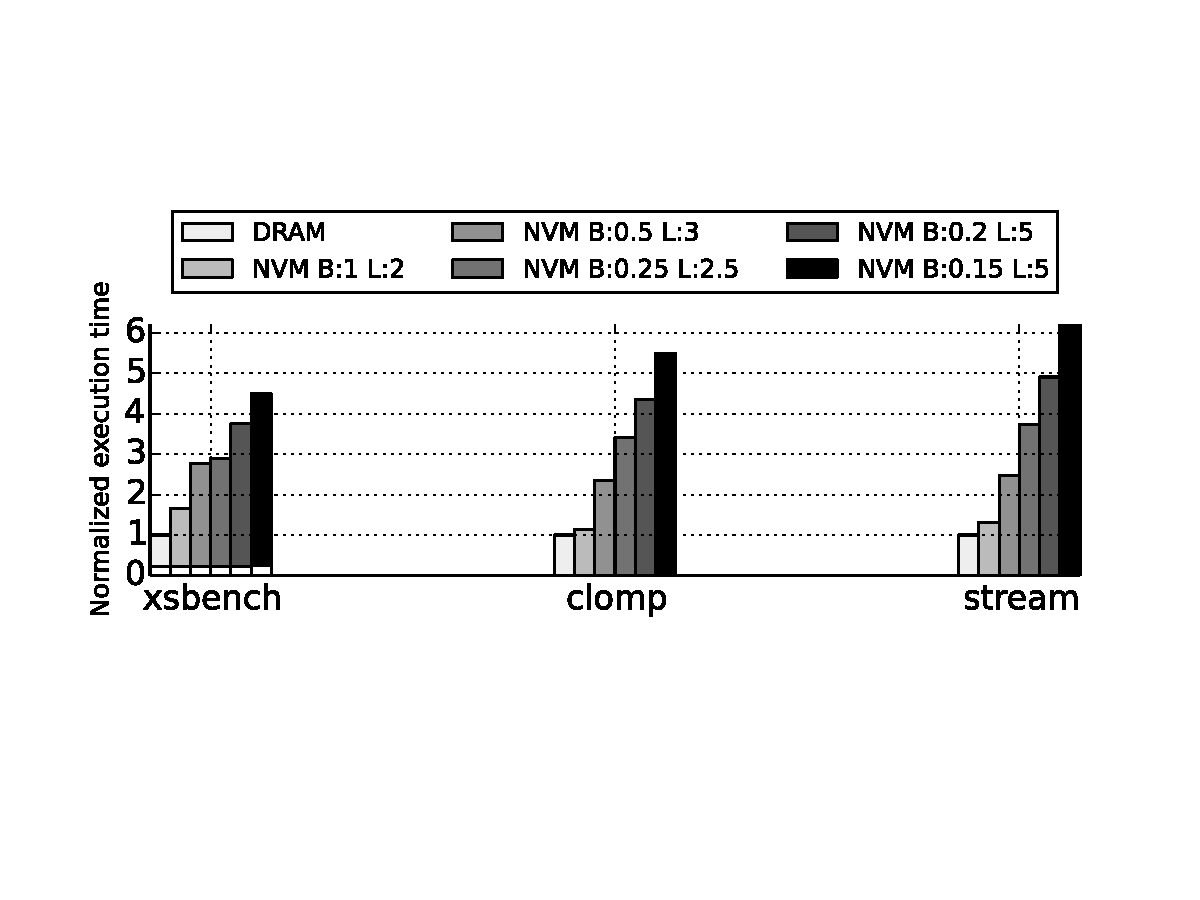
\includegraphics[width=\columnwidth]{figures/coral_throttle.pdf}
\caption{Performance slowdown across three CORAL benchmarks, normalized to `all-in-DRAM' execution. The white bottom part in XSBench shows the corresponding runtime of its initialization phase.}
\label{fig:coral_throttle}
\vspace{-0.2in}
\end{figure}

\begin{figure*}[t]
\centering
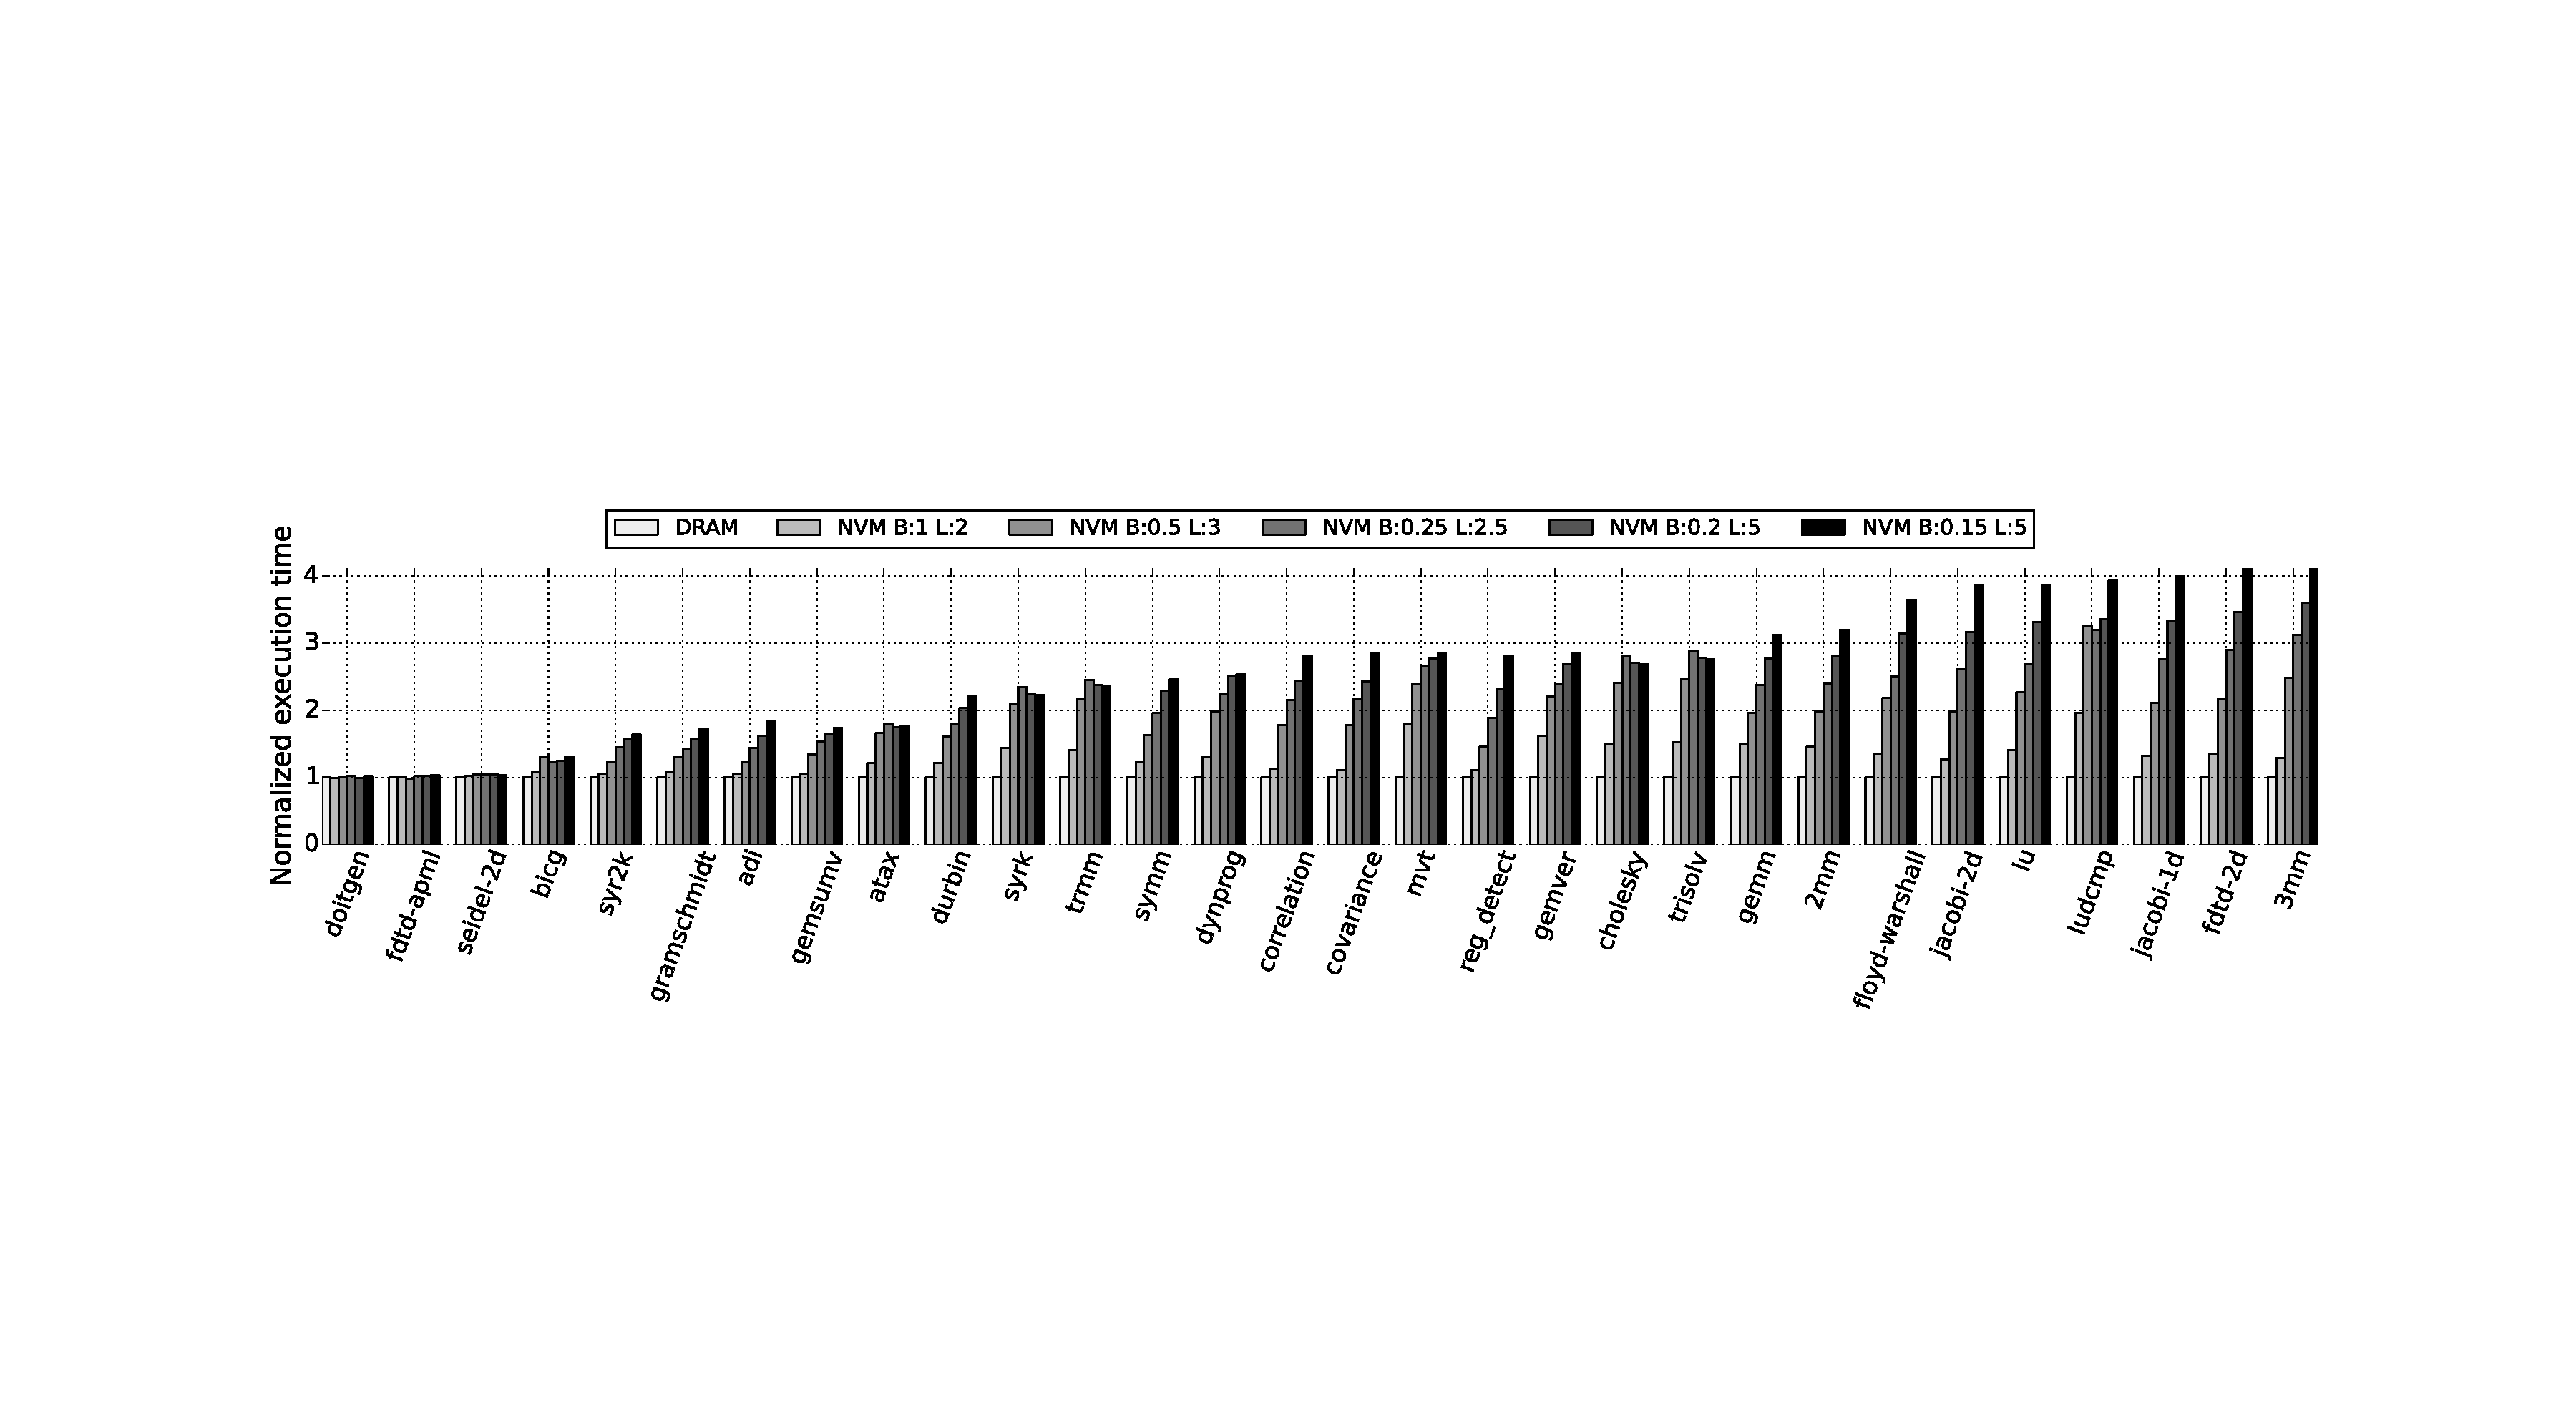
\includegraphics[width=\textwidth]{figures/polybench_throttle.pdf}
\caption{Performance slowdown across Polybench/C, normalized to `all-in-DRAM' execution.}
\label{fig:poly_throttle}
\end{figure*}

\vspace{0.6ex}
%\subsubsection
\noindent{\bf\em CORAL Experiments}
\vspace{0.3ex}

\noindent Figure ~\ref{fig:coral_throttle} shows the run time slowdown of the CORAL benchmarks when all data is allocated in SlowMem, for different combinations of bandwidth and latency, normalized to the baseline where all data lives in FastMem. We observe 
that all three applications are highly sensitive to SlowMem data allocations and accesses,  because the execution time increases when memory accesses are getting even more throttled. In the case of emulated NVM with 0.15 times less bandwidth and 5 times bigger latency, we see a 4x-6x slowdown from FastMem execution, which is very significant. 

In particular, the XSBench kernel consists of two discrete phases: the initialization phase which is run by a single thread in the beginning of execution, and the actual computation phase which is done by all 12 OpenMP threads in parallel. 
%\AG{this was very hard to see, it took me a while to realize what you were pointing to. you can use color for the bars to make it more visible, or make it all white so it stands out more explicitly. }
The white bottom part in XSBench in Figure~\ref{fig:coral_throttle} shows the total XSBench slowdown, when the computation phase is configured to have few iterations, such that the initialization phase dominates the runtime. In this case, we see that the overall application run time is not sensitive to execution over slower memory components. 



\vspace{2.0ex}

%\subsubsection
\noindent{\bf\em Polybench Experiments}
\vspace{0.3ex}

\noindent Similarly, Figure~\ref{fig:poly_throttle} shows the performance slowdown in the execution time of the Polybench suite in a setup where all data is in the available SlowMem  
(for different levels of throttled bandwidth and latency) compared to 
a baseline configuration where all data fits in FastMem.  We observe that there are kernels that 
execute up to 4x times slower in an SlowMem-only system, 
as well as others that do not get affected at all by the slower memory environment. We can classify the kernels into four distinct levels of 
sensitivity, which correspond to the degree of performance slowdown they incur, due to SlowMem-only memory accesses, as summarized in Table ~\ref{tbl:poly_class}. \\

\begin{table}[t]
\centering
{%\footnotesize
    \begin{tabular}{|p{1.4cm}|p{5.5cm}|p{0.6cm}|} \hline
	\textbf{Sensitivity \newline level} & \textbf{Kernels} & \textbf{Total} \\ \hline \hline
	None & doitgen, fdtd-apml, seidel-2d & 3/33 \\ \hline
	Low  & bicg, syr2k, gramschmidt, adi, gemsumv, atax & 6/33 \\ \hline
	Medium & durbin, syrk, trmm, symm, dynprog, correlation, covariance, mvt, reg\_detect, gemver, cholesky, trisolv & 12/33 \\ \hline
	High & gemm, 2mm, floyd-warshall, jacobi-2d, lu, ludcmp, jacobi-1d, fdtd-2d, 3mm, XSBench, CLOMP, STREAM & 12/33 \\ \hline
    \end{tabular}
}
\caption{Sensitivity classification across the 30 Polybench and 3 CORAL Benchmarks.}
\label{tbl:poly_class}
\vspace{-0.3in}
\end{table}


\noindent{\bf\em Takeaways}\\
The observation that not all applications (or some of their phases) are equally sensitive, when accessing slower memory components, can enable even more sophisticated decisions in data tiering solutions.
For example, non sensitive kernels can leverage the presence of SlowMem, allocating their entire dataset there, eliminating any need for offline profiling and finer granularity data placement decisions. 
Also, they further facilitate possible application co-running senarios, by leaving more available FastMem space for other workloads, that may have a higher sensitivity degree to SlowMem. 
More broadly, the overall sensitivity of an application is an extra parameter that needs to be taken into account when thinking about resource partitioning in shared environments. It can be used as an 
overall priority factor, when determining the amount of FastMem that each application can use, as we describe in Section ~\ref{sec:collocation}. Finally, the degree of sensitivity is also 
important to be captured for applications that have to respect Quality of Service (QoS) guarantees. It can determine the level of extra performance tuning needed to provide similar services in heterogeneous 
memory systems, compared to current DRAM-only environments.

%We can classify the kernels into three distinct categories of 
%sensitivity levels in the presence of slower memory:

%\begin{tightitemize}
%\item {\it Bandwidth sensitive}: the execution time grows linearly with the different levels of bandwidth throttling.
%\item {\it Latency sensitive}: the execution time grows linearly and shows a knee when latency does not further increase.
%\item {\it Non sensitive}: the execution time is constant across the different levels of latency and bandwidth throttling.
%\end{tightitemize}

%\begin{table}[t]
%\centering
%{\footnotesize
%    \begin{tabular}{|p{1.4cm}|p{5.5cm}|p{0.6cm}|} \hline
%		\textbf{Sensitivity \newline factor} & \textbf{Kernels} & \textbf{Total} \\ \hline \hline
%		Bandwidth & syr2k, gramschmidt, adi, gemsumv, durbin, symm, dynprog, correlation, covariance, mvt, reg\_detect, 
%					gemver, gemm, 2mm, floyd-warshall, jacobi-2d, lu, ludcmp, jacobi-1d, fdtd-2d, 3mm & 21/30 \\ \hline
%		Latency & bicg, atax, syrk, trmm, cholesky, trisolv & 6/30 \\ \hline
%		None & doitgen, fdtd-apml, seidel-2d & 3/30 \\ \hline
%    \end{tabular}
%}
%\caption{Sensitivity classification across Polybench/C.}
%\label{tbl:poly_class}
%\vspace{-0.3in}
%\end{table}

%\begin{figure*}[t]
%\centering

%    \begin{subfigure}[b]{\textwidth}
%	\includegraphics[width=\textwidth]{figures/miss_mpki.eps}
	%\end{subfigure}
    %\begin{subfigure}[b]{\textwidth}
	%\includegraphics[width=\textwidth]{figures/pref_loads.eps}
	%\end{subfigure}
    %\begin{subfigure}[b]{\textwidth}
	%\includegraphics[width=\textwidth]{figures/ipc.eps}
	%\end{subfigure}
%\caption{Performance metrics across Polybench/C.}
%\label{fig:poly_cache}
%\end{figure*}

%able~\ref{tbl:poly_class} sumarizes the classification of the different benchmarks into one of the above categories. Although the majority of kernels is bandwidth sensitive, there are few that are impacted  
%ostly by latency and others that do not get affected by any factor. 

%We next investigate whether the sensitivity of the kernels to slow memory can be easily characterized using low-level memory usage metrics such as cache use, workload size, prefetching effectiveness, etc. 
%the reasons that determine the level of sensitivity of the kernels to slow memory, looking deeper into 
%the effects of cache use, workload size and prefetching. 
%Figure~\ref{fig:poly_cache} shows the MPKI, LLC miss ratio, the number of total memory loads, the LLC prefetch miss ratio, the CPI and IPC for every benchmark in Polybench. 
%We use the Linux profiling tool \textit{perf} to extract these values for the same size of the workload used in the results shown in Figure~\ref{fig:poly_throttle}.

%Regarding the non-sensitive kernels, both \textit{doitgen} and \textit{seidel-2d} have very low MPKI values indicating this is not a memory-bound workload -- hense this classification is expected. 
%In the case of \textit{doitgen} the LLC miss ratio is 0.1\%, so the workload access pattern is cache-friendly.
%In contrast, \textit{seidel-2d} has poor cache locality with a very high LLC miss ratio, but the number of total memory load requests is low, less than 200 millions, thus 
%computation can hide the effects of not efficient cache use. For the last non-sensitive kernel, \textit{fdtd-apml}, the MPKI is not very low, rather quite larger than other kernels which do 
%exhibit sensitivity to SlowMem. However, \textit{fdtd-apml} issues a very small amount of memory load requests, around 9 million, enabling overlapped computation to 
%counter against the very poor cache locality. 

%In the case of latency sensitive kernels, the LLC miss ratio is very high, around 90\% across all of them. However, the MPKI shows great variability, as it can be as low as 1.21 in the 
%\textit{trmm} kernel or as big as 16.65 in the \textit{trisolv} kernel. A high value of MPKI usually indicates a memory intensive workload, but it is possible for a low MPKI value 
%to increase the sensitivity to latency. This is the case for \textit{trmm}, where even though the MPKI is really low, and the low CPI suggests a compute intensive workload, the number of 
%memory load requests is so big, close to 1,500 million, that ends up dominating and converting the workload to memory intensive. Additionally, 
%the access pattern of \textit{trmm} (Triangular matrix multiply) is such that doesn't allow good cache locality, as the LLC miss rate is  94.96\%, further enhancing the 
%sensitivity to latency.

%Bandwidth sensitivity is the most common one across Polybench and it can incur 1.5x up to 4x slowdown for 9x bandwidth throttling level. 
%There is a group of kernels that make very good use of the cache and prefetching having very low miss ratios, 
%such as \textit{2mm}, \textit{gemm}, \textit{gemver}, \textit{mvt}, \textit{symm}, \textit{durbin}, \textit{gramschmidt} and \textit{reg\_detect}. 
%In all these kernels the maximum slowdown will be less than 3x, indicating that good cache reuse limits the number of memory requests and 
%doesn't get impacted by the throttled bandwidth. The MPKI of these specific kernels again varies, it can be as low as 0.025 in \textit{reg\_detect} or 
%as big as 24.85 in \textit{durbin}. In the case of \textit{reg\_detect} the number of memory loads is only 500,000 and even though MPKI is so low, 
%the throttled bandwidth does impact the overall execution time.

%Thaleia: I want to sum up the observations, as well as give directions as to what metric we should choose to understand in which sensitivity level the workload belongs.
%In conclusion, we first observe that workloads which are compute intensive can benefit form the use of cache or superscalar out-of-order execution, 
%becoming resistant to slower memory accesses. In such cases, the LLC miss ratio can be misleading whereas the MPKI and workload size (number of memory load requests) can better hint the 
%potential for a non sensitive type of workload. Next, regarding the latency sensitive kernels, we notice that the LLC miss ratio is consistently high indicating potential sensitivity, 
%whereas the MPKI alone can be insufficient, as a really low MPKI value in combination with high number of load requests converts the workload to memory intensive. Finally, 
%in the case of bandwidth sensitive there are quite few kernels with very good data locality, suggesting that good cache reuse can hint sensitivity to bandwidth, and there can even be workloads 
%with very low values of MPKI and memory load requests, that get affected when running over slower memory as there is limited bandwidth they can benefit from.  \\

%\noindent{\em Summary of observations. } In summary, there are complex relationships among the application-sensitivity and these low-level events, without a clear correlation. Applying sophisticated learning methods will likely reveal greater insights, but even then building scalable models purely on low level metrics alone may be too costly, or even ineffective. 

